The Monte Carlo (MC) prediction of the nominal \ttbar + jets production samples (Powheg+Pythia8) up to six additional jets is not fully reliable. Therefore, data-based corrections, derived and applied before the fit to extract the signal, are a key ingredient in this analysis.

The two sources of mismodelling individually corrected by using data-driven correction factors. First, the rate of the \ttbar production in association with heavy-flavor jets (referred to as \ttbar +HF) is under-estimated, as observed by several previous searches and measurements. This is corrected by rescaling the normalization of each \ttbar +jets category based on the flavor of the extra jets, by comparing the yields of the data and the MC prediction in regions with different $b$-tagging requirements.

The jet multiplicity and the kinematic features of the additional jets are known to be mismodelled by the MC predictions at  multiplicity. A correction is then deployed by applying reweighting factors on the mismodelled observables, derived by comparing their distributions between the data and the MC prediction in the 2b region.
In this second step, a neural network-based approach is used to estimate the probability density functions of the data and the MC prediction, to derive reweighting factor as a ratio of them. This method allows to correct multiple observables at the same time, thus the MVA strategy used to define a signal-to-background discriminant has further flexibility on the input features choice as their modelling will typically be corrected.

%\subsection{\ttbar + jets truth classification}

\subsection{Flavor rescaling}
\label{sec:hf_rew}
The flavor rescaling corrects the under-estimation of the $\ttbar+HF$ production rate in the MC prediction. This is performed by rescaling the normalization of $\ttbar+light$ (TTL), $\ttbar+\ge 1c$ (TTC) and $\ttbar+\ge 1b$ (TTB). The scale factors are derived by performing a likelihood fit on the sum of the pseudo continuous b-tagged score (pcb) of the third and forth jets ranked in DL1r score, as this variable is highly sensitive to the $\ttbar+HF$ samples. A combined fit is performed in 7j region from the 1L channel and 5j region from the OS channel with $=2b$, $=3b$ and $\geq 4b$ requirements, where the signal contamination of all the signal mass points is around or smaller than $0.1\%$. The normalisation of TTL, TTC and TTB are free floating in this fit, and that TTL normalisation for 1L and 2LOS are treated as two independent normalisaiton factors. The nominal \ttbar sample is used for this fit. The nuisance parameters associated to the systematic uncertainties on the b-tagging efficiency (as described in Section~\ref{b-tagging_uncertianties}) and the cross-section uncertainties of other backgrounds, which cannot be neglected in the fitting regions, are fitted together with the correction factors of TTL, TTC and TTB because these uncertainties highly affect the yields of $\ttbar+HF$ and other backgrounds.

% as given in the Table~\ref{tab:HF_postFit_nominal}

\begin{table}[th!]
    \centering
    \def\arraystretch{1.2}
    \resizebox*{0.3\textwidth}{!}{
    \begin{tabular}{c|cc}
        \toprule
          & 1L & OS \\
          & $=7j$ & $=5j$ \\
        \hline
         2b & $<0.1\%$ & $<0.1\%$ \\
         3b & $<0.1\%$ & $<0.1\%$ \\
         $\geq4b$ & $0.2\%$ & $0.1\%$ \\
        \bottomrule
    \end{tabular}
    }
    \caption{\label{tab:sigContam_HFCorrRegion}The signal (BSMtttt M700) over background ratio in each of the regions used to derive the HF rescaling factors before any scaling applied.}
\end{table}

The pre-fit and post-fit distributions of the third and the forth jets pcb sum in 1L and OS channels can be found in figure~\ref{fig:1L_pcb34_PrePost} and~\ref{fig:2LOS_pcb34_PrePost} respectively. The pre-fit and post-fit summary plots, which show the yields in each region, in both channel can be found in figure~\ref{fig:HF_summaryPlot} while the fitted normalization factors and nuisance parameters can be found in figure~\ref{fig:HF_scale_fit}. The obtained normalization factors are consistent with other ATLAS analyses targeting similar phase space. For example, the ttH(bb) measurement \cite{HIGG-2017-03} found tt+b and tt+c normalization factors of 1.24 and 1.63, respectively. Most of the nuisance parametrs are neither pulled nor constrained. However, when the fits are done separately on two channels, it is observed that both nuisance parameters of c-tagging EV0 and light-tagging EV0 are pulled in oposite direction between two channels. Therefore these two nuisance parameters are decorrelated from the two channels in the combined fit.
It is also found that having the combined fit in TTL scale factor causes the inconsistent results with the 1L and OS channel separated fit, because the acceptance of the TTL events between these two channel are different. To keep a stable fit results, the TTL correction factors are derived on separate channels during the combined fit.



\begin{figure}[!htb]
    \centering
    \subfloat[1L$(=7j,=2b)$ Pre-fit]{
        
\includegraphics[height=0.3\textheight]{plots/bkg_modelling/HF_scaling/pcbSum34_ljets_7j2b_preFit.pdf}
    }
    \subfloat[1L$(=7j,=2b)$ Post-Fit]{
        
\includegraphics[height=0.3\textheight]{plots/bkg_modelling/HF_scaling/pcbSum34_ljets_7j2b_postFit.pdf}
    }

    \subfloat[1L$(=7j,=3b)$ Pre-fit]{
        
\includegraphics[height=0.3\textheight]{plots/bkg_modelling/HF_scaling/pcbSum34_ljets_7j3b_preFit.pdf}
    }
    \subfloat[1L$(=7j,=3b)$ Post-Fit]{
        
\includegraphics[height=0.3\textheight]{plots/bkg_modelling/HF_scaling/pcbSum34_ljets_7j3b_postFit.pdf}
    }
    
    \subfloat[1L$(=7j,\geq 4b)$ Pre-fit]{
        
\includegraphics[height=0.3\textheight]{plots/bkg_modelling/HF_scaling/pcbSum34_ljets_7jge4b_preFit.pdf}
    }
    \subfloat[1L$(=7j,\geq 4b)$ Post-Fit]{
        
\includegraphics[height=0.3\textheight]{plots/bkg_modelling/HF_scaling/pcbSum34_ljets_7jge4b_postFit.pdf}
    }
    \caption{\label{fig:1L_pcb34_PrePost}The pre-fit (left) and post-fit (right) distributions of pcb sum of the third and the forth jets at 7j region with $=2b$, $=3b$ and $\geq 4b$ in 1L channel to derive the HF scale factor.}
\end{figure}


\begin{figure}[!htb]
    \centering
    \subfloat[1L$(=5j,=2b)$ Pre-fit]{
        
\includegraphics[height=0.3\textheight]{plots/bkg_modelling/HF_scaling/pcbSum34_os2l_5j2b_preFit.pdf}
    }
    \subfloat[1L$(=5j,=2b)$ Post-Fit]{
        
\includegraphics[height=0.3\textheight]{plots/bkg_modelling/HF_scaling/pcbSum34_os2l_5j2b_postFit.pdf}
    }

    \subfloat[1L$(=5j,=3b)$ Pre-fit]{
        
\includegraphics[height=0.3\textheight]{plots/bkg_modelling/HF_scaling/pcbSum34_os2l_5j3b_preFit.pdf}
    }
    \subfloat[1L$(=5j,=3b)$ Post-Fit]{
        
\includegraphics[height=0.3\textheight]{plots/bkg_modelling/HF_scaling/pcbSum34_os2l_5j3b_postFit.pdf}
    }

    \subfloat[1L$(=5j,\geq 4b)$ Pre-fit]{
        
\includegraphics[height=0.3\textheight]{plots/bkg_modelling/HF_scaling/pcbSum34_os2l_5jge4b_preFit.pdf}
    }
    \subfloat[1L$(=5j,\geq 4b)$ Post-Fit]{
        
\includegraphics[height=0.3\textheight]{plots/bkg_modelling/HF_scaling/pcbSum34_os2l_5jge4b_postFit.pdf}
    }
    \caption{\label{fig:2LOS_pcb34_PrePost}The pre-fit (left) and post-fit (right) distributions of pcb sum of the third and the forth jets at 5j region with $=2b$, $=3b$ and $\geq 4b$ in OS channel to derive the HF scale factor.}
\end{figure}

\begin{figure}[ht!]
  \centering
    \begin{subfigure}[t]{\textwidth}
        \centering
        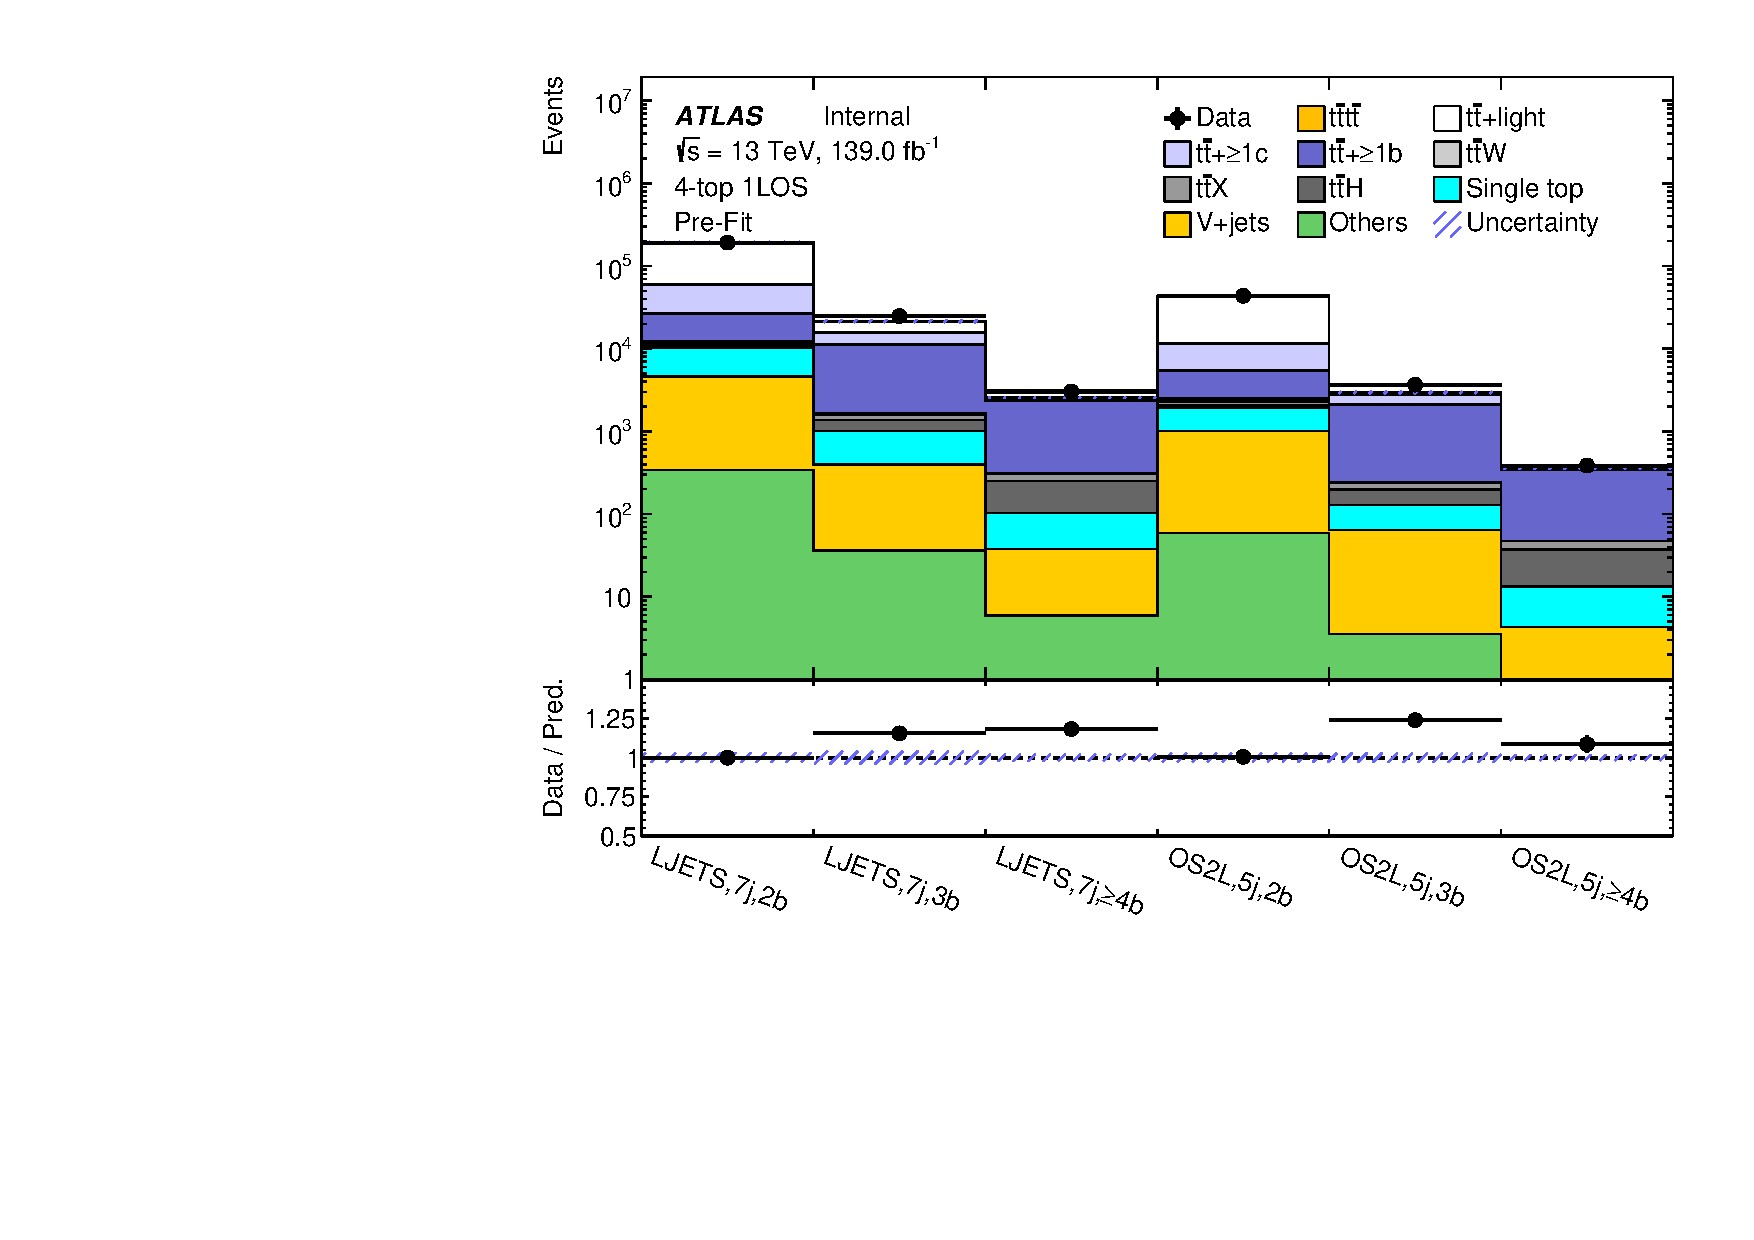
\includegraphics[width=0.48\textwidth]{plots/bkg_modelling/HF_scaling/Summary_preFit.pdf}
        
\includegraphics[width=0.48\textwidth]{plots/bkg_modelling/HF_scaling/Summary_postFit.pdf}
    \end{subfigure}
    \caption{Pre-fit (left) and post-fit (right) distributions of the yields in the regions included in the fit to determine HF scale factors.}
    \label{fig:HF_summaryPlot}
\end{figure}

\begin{figure}[ht!]
  \centering
    \begin{subfigure}[t]{\textwidth}
        \centering
        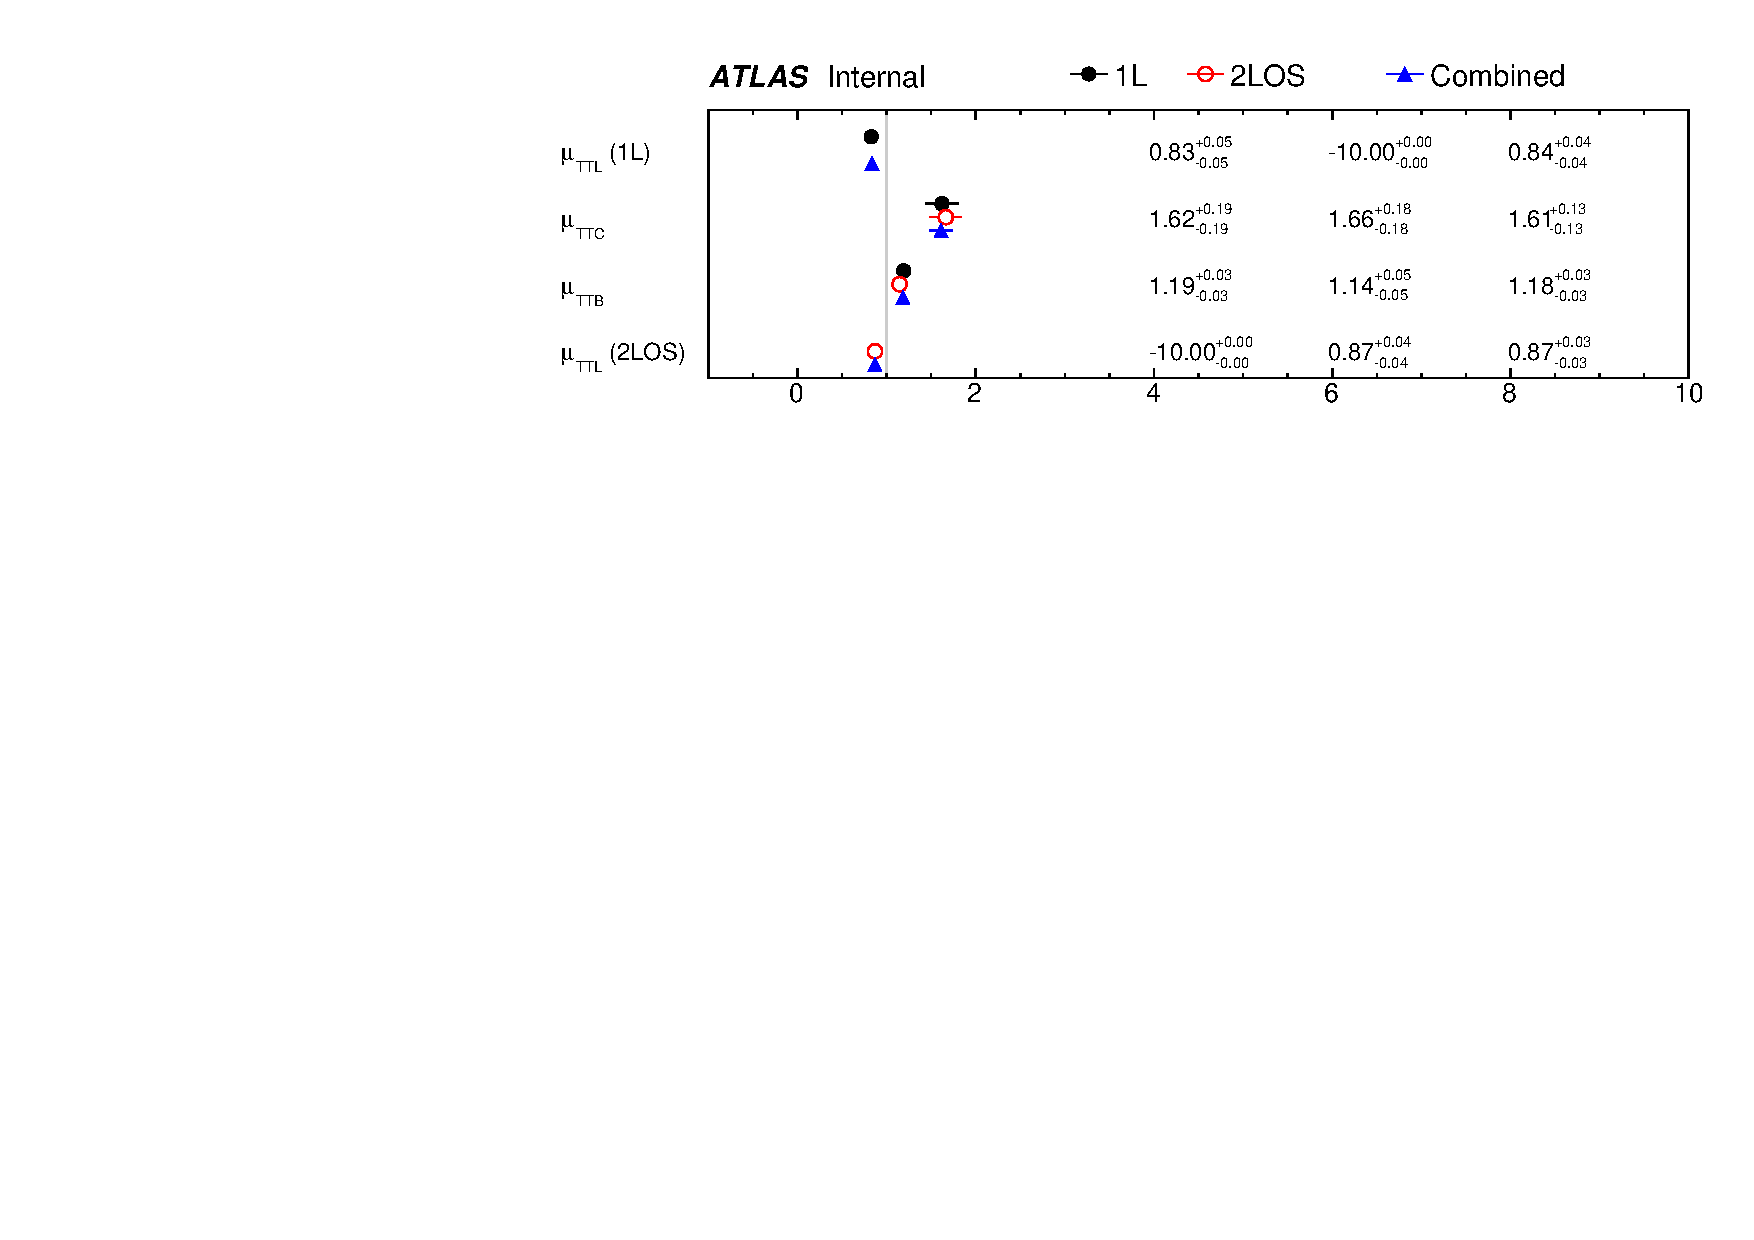
\includegraphics[width=0.78\textwidth]{plots/bkg_modelling/HF_scaling/NormFactors_multiFit.pdf}
    \end{subfigure}
    \bigskip
    \centering
    \begin{subfigure}[t]{\textwidth}
        \centering
        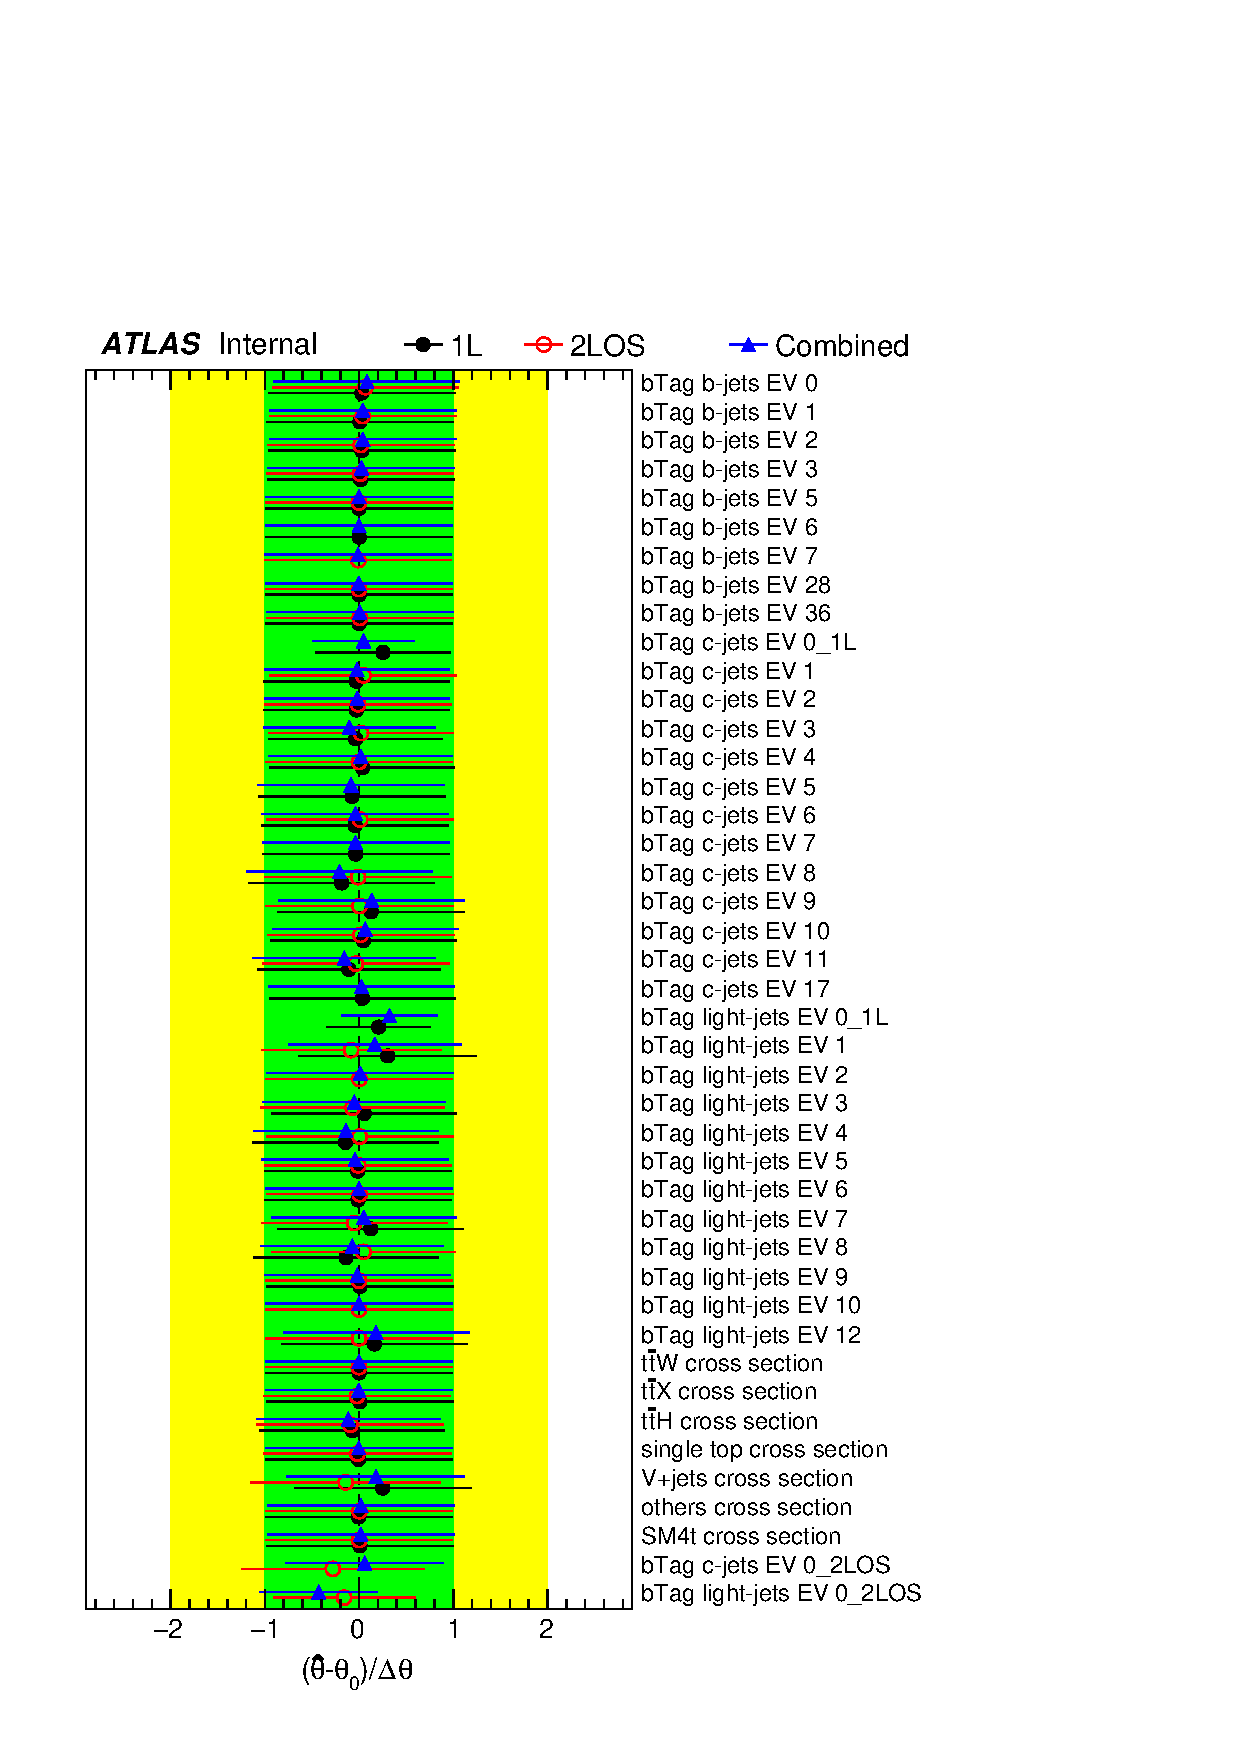
\includegraphics[width=0.58\textwidth]{plots/bkg_modelling/HF_scaling/PullPlots_multiFit.pdf}
    \end{subfigure}
    \caption{Fitted normalisation factors and nuisance parameters. Black, red and blue color refer to 1L, OS and combined channel fit respectively.}
    \label{fig:HF_scale_fit}
\end{figure}



The HF scale factors used in this analysis for the nominal \ttbar sample are taken as the normalization factors from Figure \ref{fig:HF_scale_fit}. It was found that the ratio $\ttbar_{postfit}^{nominal} / \ttbar_{prefit}^{nominal}$ based on Tables~\ref{tab:HF_preFit} and \ref{tab:HF_postFit_nominal} is very similar to the obtained normalization factors (1.18 for \ttbin, 1.60 for \ttcin, 0.83 for TTL (1L), and  0.87 for TTL (2L)).

The HF scale factors for the alternative \ttbar\ samples are obtained as the ratio $\ttbar_{postfit}^{nominal} / \ttbar_{prefit}^{alternative}$ based on the Tables~\ref{tab:HF_preFit} and \ref{tab:HF_postFit_nominal}. This is the preferred option because it also contains effects from the pulls from all nuisance parameters (it makes no difference for the nominal sample). No separate fits with alternative samples were used because they lead to large pulls on several nuisance parameters.  The HF scale factors of different \ttbar samples are summarized in table~\ref{tab:HF_results}. The \ttbar modelling systematics obtained using alternative weights in the nominal \ttbar sample (FSR, ISR, renormalization and factorization scale) are using the HF scale factors for the nominal \ttbar sample (the differences are negligible as documented in Appendix \ref{app:HFweights_weightSystematics}).


\begin{table}[!htb]
    \centering
    \resizebox*{0.72\textwidth}{!}{
    \begin{tabular}{c|c|c|c||c}
        \hline \hline
        \multicolumn{5}{c}{\textbf{Pre-fit 1L (Nominal)}}\\
        \hline
        & $LJETS,7j,2b$ & $LJETS,7j,3b$ & $LJETS,7j,\geq 4b$ & Total \\
        \hline 
TTL &  $132532.64 \pm 4215.99 $ & $5751.48 \pm 470.26$ & $44.24 \pm 11.26$ & $138328.36 \pm 4242.15$\\
TTC & $32634.67 \pm 888.81$ & $4491.35 \pm 360.70$ & $181.26 \pm 27.45$ & $37307.28 \pm 959.60$ \\
TTB & $14525.10 \pm 17.06$ & $9577.63 \pm 12.25$ & $2016.50 \pm 4.30$ & $26119.23 \pm 21.44$ \\ 
        \hline \hline
        \multicolumn{5}{c}{\textbf{Pre-fit OS (Nominal)}}\\
        \hline
        & $OS2L,5j,2b$ & $OS2L,5j,3b$ & $OS2L,5j,\geq 4b$ & Total \\
        \hline 
TTL &  $31869.24 \pm 961.92$ & $189.42 \pm 38.91$ & $0.51 \pm 0.26$ & $32059.17 \pm 962.71$\\
TTC & $6015.13\pm 150.02$ & $645.69 \pm 52.96$ & $10.95 \pm 1.71$ & $6671.77 \pm 159.10$  \\
TTB & $2994.50 \pm 5.91$ & $1870.36 \pm 4.24$ & $296.20 \pm 1.36$ & $5161.06 \pm 7.40$ \\
        \hline \hline \hline
        \multicolumn{5}{c}{\textbf{Pre-fit 1L (ttbb 4FS)}}\\
        \hline
        & $LJETS,7j,2b$ & $LJETS,7j,3b$ & $LJETS,7j,\geq 4b$ & Total \\
        \hline
TTL &  $132532.64 \pm 4215.99 $ & $5751.48 \pm 470.26$ & $44.24 \pm 11.26$ & $138328.36 \pm 4242.15$\\
TTC & $32634.67 \pm 888.81$ & $4491.35 \pm 360.70$ & $181.26 \pm 27.45$ & $37307.28 \pm 959.60$ \\
TTB & $14395.47 \pm 27.52$ & $9852.50 \pm 22.34$ & $2180.87 \pm 10.15$ & $26428.84 \pm 36.87$ \\
        \hline \hline
        \multicolumn{5}{c}{\textbf{Pre-fit OS (ttbb 4FS)}}\\
        \hline
         & $OS2L,5j,2b$ & $OS2L,5j,3b$ & $OS2L,5j,\geq 4b$ & Total \\
        \hline
TTL &  $31869.24 \pm 961.92$ & $189.42 \pm 38.91$ & $0.51 \pm 0.26$ & $32059.17 \pm 962.71$\\
TTC & $6015.13\pm 150.02$ & $645.69 \pm 52.96$ & $10.95 \pm 1.71$ & $6671.77 \pm 159.10$  \\
TTB & $2898.23 \pm 9.00$ & $1843.86 \pm 6.87$ & $309.36 \pm 2.65$ & $5051.45 \pm 11.63$ \\
        \hline \hline \hline
        \multicolumn{5}{c}{\textbf{Pre-fit 1L (aMcAtNloPy8)}}\\
        \hline
        & $LJETS,7j,2b$ & $LJETS,7j,3b$ & $LJETS,7j,\geq 4b$ & Total \\
        \hline
TTL & $117273.46 \pm 3716.78$ & $5116.16 \pm 420.24$ & $38.65 \pm 10.28$ & $122428.27 \pm 3740.48$\\
TTC & $29348.28 \pm 809.43$ & $3924.70 \pm 314.28$ & $151.22 \pm 22.69$ & $33424.20 \pm 868.60$  \\
TTB & $13398.83 \pm 38.45$ & $8851.56 \pm 27.21$ & $1913.43 \pm 8.88$ & $24163.82 \pm 47.93$ \\
        \hline \hline
        \multicolumn{5}{c}{\textbf{Pre-fit OS (aMcAtNloPy8)}}\\
        \hline
        & $OS2L,5j,2b$ & $OS2L,5j,3b$ & $OS2L,5j,\geq 4b$ & Total \\
        \hline
TTL &  $28880.01 \pm 889.56$ & $160.68 \pm 33.08$ & $0.72 \pm 0.40$ & $29041.41 \pm 890.17$ \\
TTC & $5565.00 \pm 140.81$ & $593.38 \pm 48.86$ & $9.58 \pm 1.60$ & $6167.96 \pm 149.05$\\
TTB & $2828.95 \pm 11.79$ & $1772.51 \pm 8.41$ & $296.82 \pm 2.72$ & $4898.28 \pm 14.74$\\
        \hline \hline \hline
        \multicolumn{5}{c}{\textbf{Pre-fit 1L (PhHerwig)}}\\
        \hline 
 & $LJETS,7j,2b$ & $LJETS,7j,3b$ & $LJETS,7j,\geq 4b$ & Total \\
        \hline
TTL & $166159.84 \pm 5232.84$ & $7001.95 \pm 573.57$ & $52.10 \pm 13.60$ & $173213.89 \pm 5264.20$ \\
TTC & $23306.84 \pm 635.75$ & $3190.58 \pm 255.02$ & $125.72 \pm 18.59$ & $26623.14 \pm 685.24$ \\
TTB & $11965.54 \pm 19.36$ & $7104.79 \pm 13.27$ & $1346.67 \pm 4.30$ & $20417.00 \pm 23.86$ \\ 
        \hline \hline
        \multicolumn{5}{c}{\textbf{Pre-fit OS (PhHerwig)}}\\
        \hline
 & $OS2L,5j,2b$ & $OS2L,5j,3b$ & $OS2L,5j,\geq 4b$ & Total \\
        \hline
TTL & $38019.17 \pm 1160.60$ & $199.01 \pm 40.78$ & $0.95 \pm 0.46$ & $38219.13 \pm 1161.32$ \\
TTC & $4689.39 \pm 118.92$ & $494.01 \pm 40.09$ & $7.17 \pm 1.09$ & $5190.57 \pm 125.50$ \\
TTB & $1845.12 \pm 5.22$ & $1184.89 \pm 3.62$ & $204.56 \pm 1.20$ & $3234.57 \pm 6.46$ \\ 
       \hline \hline
    \end{tabular}
    }
    \caption{\label{tab:HF_preFit}The pre-fit yields before the HF rescaling fit of different MC samples.}\end{table}

\begin{table}[!htb]
    \centering
    \resizebox*{0.72\textwidth}{!}{
    \begin{tabular}{c|c|c|c||c}
        \hline \hline
        \multicolumn{5}{c}{\textbf{Post-fit 1L (Nominal)}}\\
        \hline
        & $LJETS,7j,2b$ & $LJETS,7j,3b$ & $LJETS,7j,\geq 4b$ & Total \\
        \hline
TTL &  $109830.98 \pm 4123.96$ & $4709.29\pm 186.97$ & $34.41 \pm 2.65$ & $114574.68 \pm 4128.20$ \\
TTC & $52241.19 \pm 4105.77$ & $7145.79 \pm 557.11$ & $286.59 \pm 22.83$ & $59673.57 \pm 4143.46$ \\
TTB & $17153.71 \pm 403.20$ & $11310.90 \pm 265.87$ & $2381.43 \pm 55.98$ & $30846.04 \pm 486.20$\\
        \hline \hline
        \multicolumn{5}{c}{\textbf{Post-fit OS (Nominal)}}\\
        \hline
        & $OS2L,5j,2b$ & $OS2L,5j,3b$ & $OS2L,5j,\geq 4b$ & Total \\
        \hline
TTL & $27717.06 \pm 794.56$ & $178.53 \pm 26.36$ & $0.53 \pm 0.18$ & $27896.12 \pm 795.00$\\
TTC &  $9707.14 \pm 703.54$ & $1039.12 \pm 63.97$ & $17.83 \pm 1.62$ &  $10764.09 \pm 706.44$ \\
TTB & $3536.52 \pm 83.14$ & $2208.95 \pm 51.92$ & $349.84 \pm 8.24$ & $6095.31 \pm 98.37$ \\
        \hline \hline
    \end{tabular}
    }
    \caption{\label{tab:HF_postFit_nominal}The post-fit yields after the HF rescaling fit on the nominal MC samples.}
\end{table}

\begin{table}[!htb]
    \centering
    \resizebox*{0.5\textwidth}{!}{
    \begin{tabular}{c|cccc}
        \hline \hline
        & TTL (1L) & TTL (OS) & TTC & TTB \\
        Nominal & $0.84\pm 0.04$ & $0.87\pm 0.03$ & $1.61\pm 0.13$ & $1.18\pm 0.03$\\
        ttbb 4FS & $0.83\pm 0.04$ & $0.87\pm 0.04$ & $1.60\pm 0.10$ & $1.17\pm 0.02$ \\
        aMcAtNloPy8 & $0.94\pm 0.04$ & $0.96\pm 0.04$ & $1.78\pm 0.11$ & $1.27\pm 0.01$\\
        PhHerwig & $0.66\pm 0.03$ & $0.73\pm 0.03$ & $2.21\pm 0.14$ & $1.56\pm 0.02$ \\ 
        \hline \hline
    \end{tabular}
    }
    \caption{\label{tab:HF_results}The summary of HF scale factors of TTL (1L and OS), TTC and TTB of different \ttbar+jets MC samples.}
\end{table}



\clearpage
%%%%
\subsection{Neural-network based kinematic reweighting}
\label{sec:nn_rew}
After applying the HF scale factors derived in the previous subsection, a kinematic reweighitng is derived using a neural network. The kinematic reweighting is based on estimating a probability density function (p.d.f.) in an n-dimensional space by using a feed-forward classification neural network~\cite{nn_pdfs}. The output of a neural network trained to disentangle between two classes has a probabilistic interpretation in terms of the a-posteriori Bayesian probability. This can be used to approximate p.d.f. of the both class.

\begin{equation}
  o^{min}({\bf x}) = P(data|{\bf x}) = \dfrac{\alpha_{data}P_{data}({\bf x})}{\alpha_{data}P_{data}({\bf x})+\alpha_{MC}P_{MC}({\bf x})}
\end{equation}

where $o$ is NN output, ${\bf x}$ is input vector, $\alpha_{data}$ and $\alpha_{MC}$ are the proportions of each class of events used for training, satisfying $\alpha_{data} + \alpha_{MC} = 1$.

From the above equation, it is straightforward to extract reweighting factor as a ratio of two p.d.f.

\begin{equation}
  w({\bf x}) = \dfrac{\alpha_{data}P_{data}({\bf x})}{\alpha_{MC}P_{MC}({\bf x})} = \dfrac{o({\bf x})}{1-o({\bf x})}
  \label{rew::1l}
\end{equation}

Therefore the reweighting can be derived in ${\bf x}$ space for each event in an unbinned way. The both data and MC here refering to $\ttbar +jets$. To subtract non-\ttbar MC samples from the data, non-\ttbar MC samples are included in to the training with a data label, but by using a negative event weight. Then the final expression is still valid in the same form.

The training region is defined in $7j (5j)$ and $2b$ for 1L (2LOS). The neural network is fed by each jet $p_T$, number of jets and reclustered jets, missing $E_T$ and lepton jet $p_T$. The goal here is not only correcting these kinematics but also the kinematics derived from them.

With respect to all of the above, we modified loss function with an exponential loss function, therefore, reweighting factor is defined differently.
The motivation of this modification is due to some studies showing better performance especially in the case of low statistics~\cite{moustakides2019training}.


\begin{equation}
  \mathcal{L} = P_{data}e^{-o({\bf x})/2}+P_{MC}e^{o({\bf x})/2} \\
  \dfrac{d\mathcal{L}}{do({\bf x})} = -\dfrac{P_{data}}{2}e^{-o({\bf x})/2}+\dfrac{P_{MC}}{2}e^{o({\bf x})/2} = 0
\end{equation}

from this equation, reweighting factor can be derived as following,

\begin{equation}
  w({\bf x}) = e^{o({\bf x})}
\end{equation}

In addition to changing loss function, learning rate decay has been used during the training, and an early stop mechanism developed based on the minimization of loss function after each epoch.

Training has been performed on the \ttbar+jets nominal and alternative samples independently. So each sample was corrected by their own training. A generic feed-forward architecture found by a hyper-parameter scan for all trainings.

The kinematic reweighting on $H_T$ distribution is illusturated in Figure~\ref{fig::cor1l}. More discussion in Appendices~\ref{app:background_modeling_comp} and \ref{app:NNRewPlots}. It is expected that the kinematic reweighting does not change the normalization, only the shape. This was verified in Table~\ref{tab:Rew_NoRew_YieldsRatio}.

\begin{itemize}
\item Minimizer : Stochastic Gradient Descent
\item Learning Rate : 0.0036 and Momentum : 0.9
\item Loss function : Binary cross entropy / exponential
\item Architecture : 4ReLU(30)xTanh(30)xLinear(1)
\item Mini Batch size : 1000
\item Epoch : early stopping around 250 epoch
\end{itemize}

\begin{figure}[!htb]
  \centering
    \begin{subfigure}[t]{\textwidth}
        \centering
        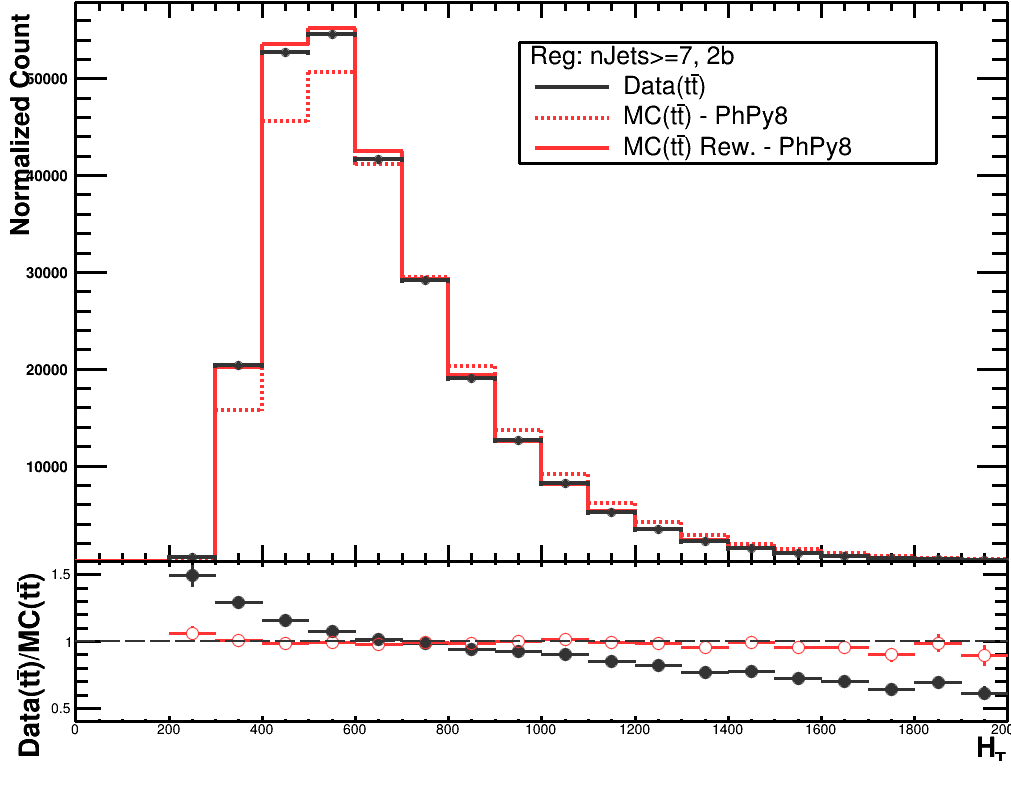
\includegraphics[width=0.48\textwidth]{plots/bkg_modelling/cor_1l_nom.png}
        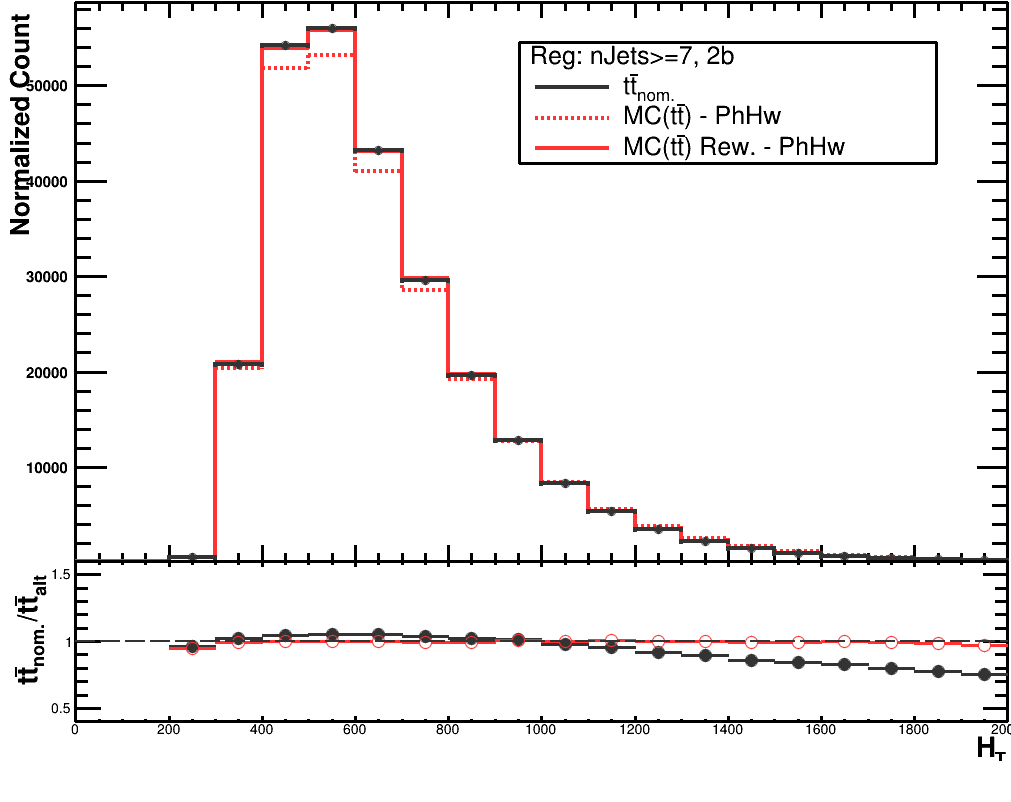
\includegraphics[width=0.48\textwidth]{plots/bkg_modelling/cor_1l_alt.png}
    \end{subfigure}
    \caption{The kinematic reweighting effect on $H_T$ distribution, and data/MC ratio for 1L \ttbar+jets nominal and one of the alternative samples. The black points in the ratio plot refer to data/MC ratio for the nominal MC samples with HF reweighting but without kinematic reweighting. The red points of the ratio plot refer to the data/MC ratio for the nominal MC samples after both HF and kinematic reweighting have been applied.}
    \label{fig::cor1l}
\end{figure}


\subsubsection{Uncertainty Propagation for NN Reweighting}
\label{sec:NN_reweighting:uncertainty}

Two additional uncertainties are considered to take into account the uncertainty on the data-driven
corrections. The reweighting factors on \ttbar + jets depend on the size of the non-\ttbar processes subtracted from data.
The cross section of the non-\ttbar processes is therefore varied by $\pm 50\%$ and alternative reweighting
factors are derived. The resulting difference in the final distribution is taken as a nuisance parameter in the
likelihood fit. The effect of this uncertainty ranges from 3\% to 4\%.

Understanding the influence of statistical uncertainty on background modeling aids in calibrating adjustments to the data within the fitted distributions.
Among the array of available methods in the literature, the Monte Carlo (MC) dropout method~\cite{gal2016dropout} was selected for its straightforward implementation and its flexibility in 
accommodating diverse neural network architectures. The dropout is originally a regularization method for neural networks where randomly selected neurons are ignored during training.
To apply this method following steps are considered,

\begin{itemize}
    \item {\bf Standard training:} Initialy a neural network is trained for reweighting factors without implementation of dropout layers.
    \item {\bf Dropout training:} A second training is considered with implementation of dropout layers into same architecture of standard training.
    \item {\bf Dropout evaluation:} The neural network from the dropout training is evaluated 1000 times by keep using dropout layers, so the random drops of neurons still remain, and results varied up in each iteration.
    \item {\bf Uncertainty propagation:} The standard deviation is calculated from the varied results of dropout evaluation. 
\end{itemize}


This method has been tested via toy and real data to understand better to effect of statistics on uncertainty.
For this example, we have created two different exponential distributions and matched them to each other through the neural network reweighting, and a fit function.
The uncertainty from the MC dropout method and the confidence interval at 68\% from the fit are compared in Figure~\ref{fig::unc_rew}, for poor and high statistics.
A similar test has been done on the training region by selecting different multiplicity of number of jets to observe how statistical fluctuation is effecting on this method in Figure~\ref{fig::unc_rew_real}

\begin{figure}[!htb]
    \centering
      (a)
      \begin{subfigure}[t]{\textwidth}
          \centering
          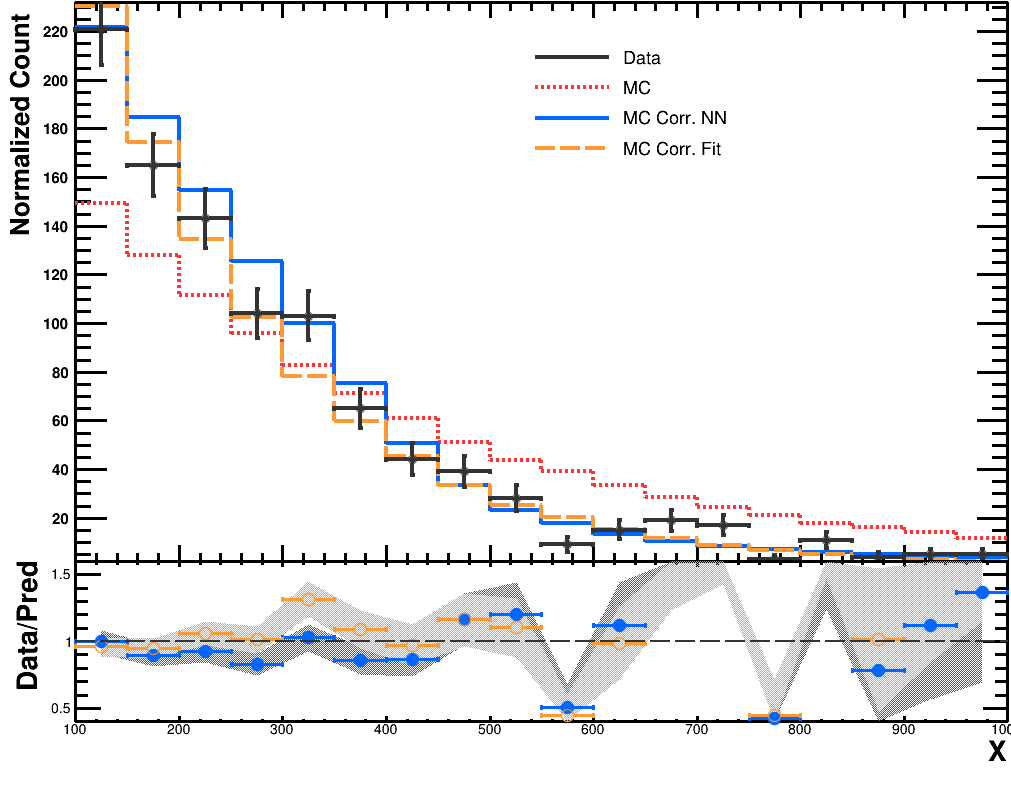
\includegraphics[width=0.48\textwidth]{plots/bkg_modelling/toy_poor.png}
          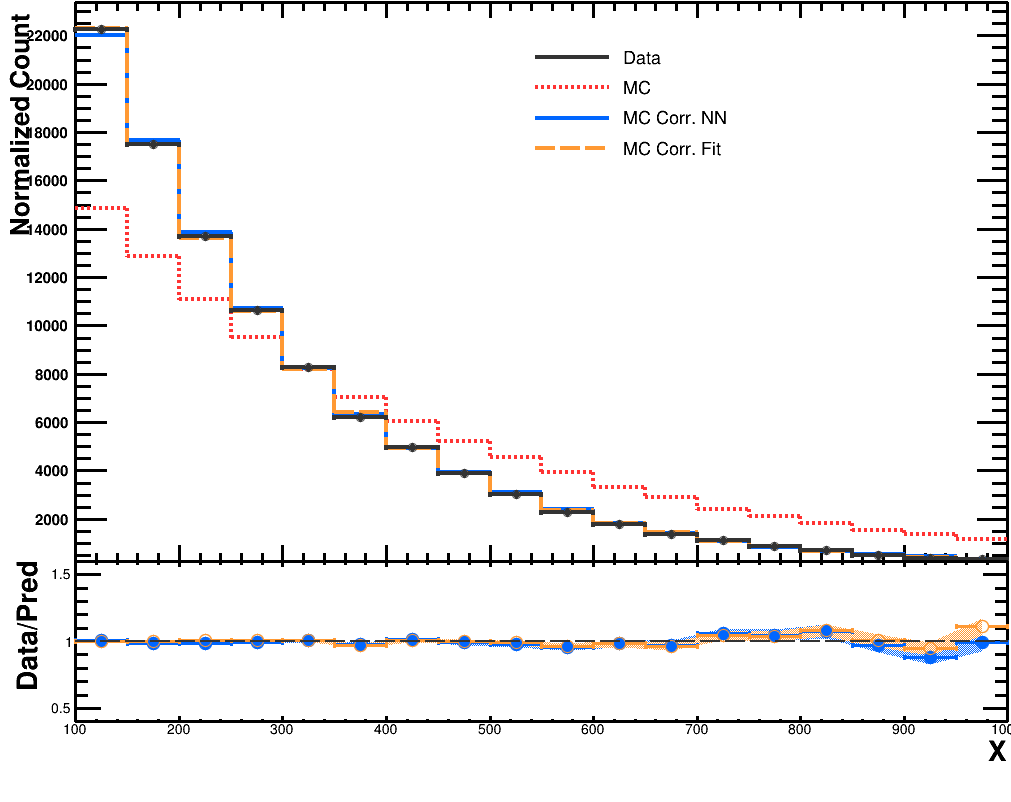
\includegraphics[width=0.48\textwidth]{plots/bkg_modelling/toy.png}
      \end{subfigure}
      (b)
      \begin{subfigure}[t]{\textwidth}
        \centering
        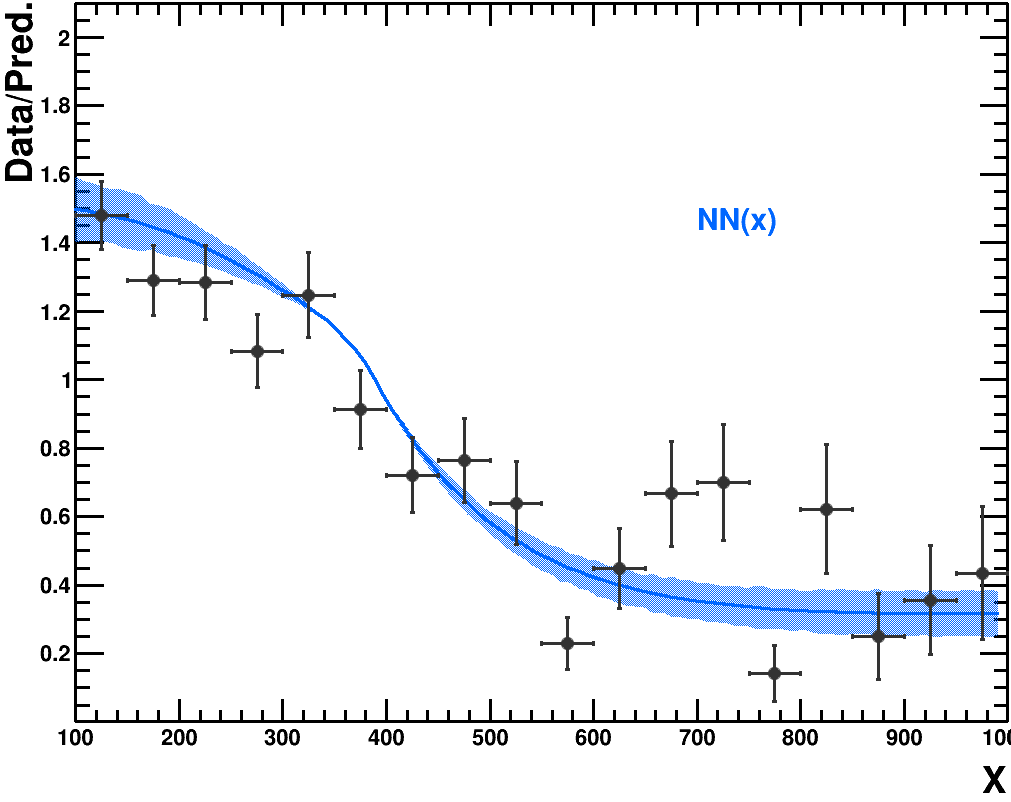
\includegraphics[width=0.48\textwidth]{plots/bkg_modelling/toy_nn_poor.png}
        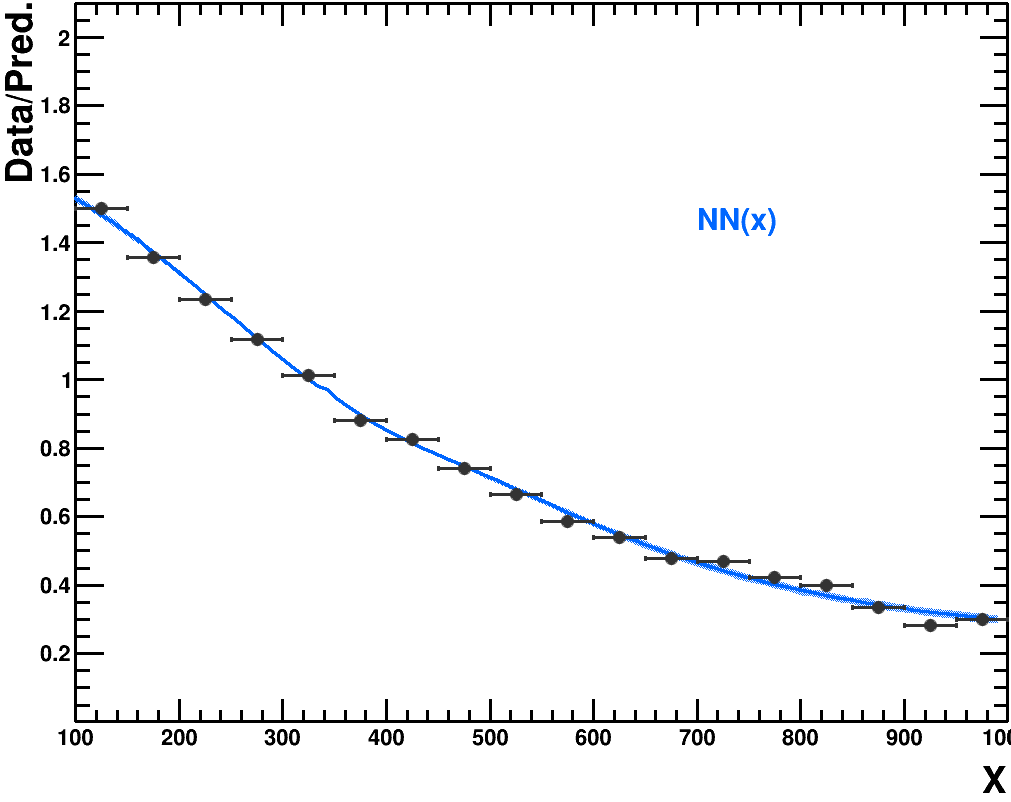
\includegraphics[width=0.48\textwidth]{plots/bkg_modelling/toy_nn.png}
      \end{subfigure}
      (c)
      \begin{subfigure}[t]{\textwidth}
        \centering
        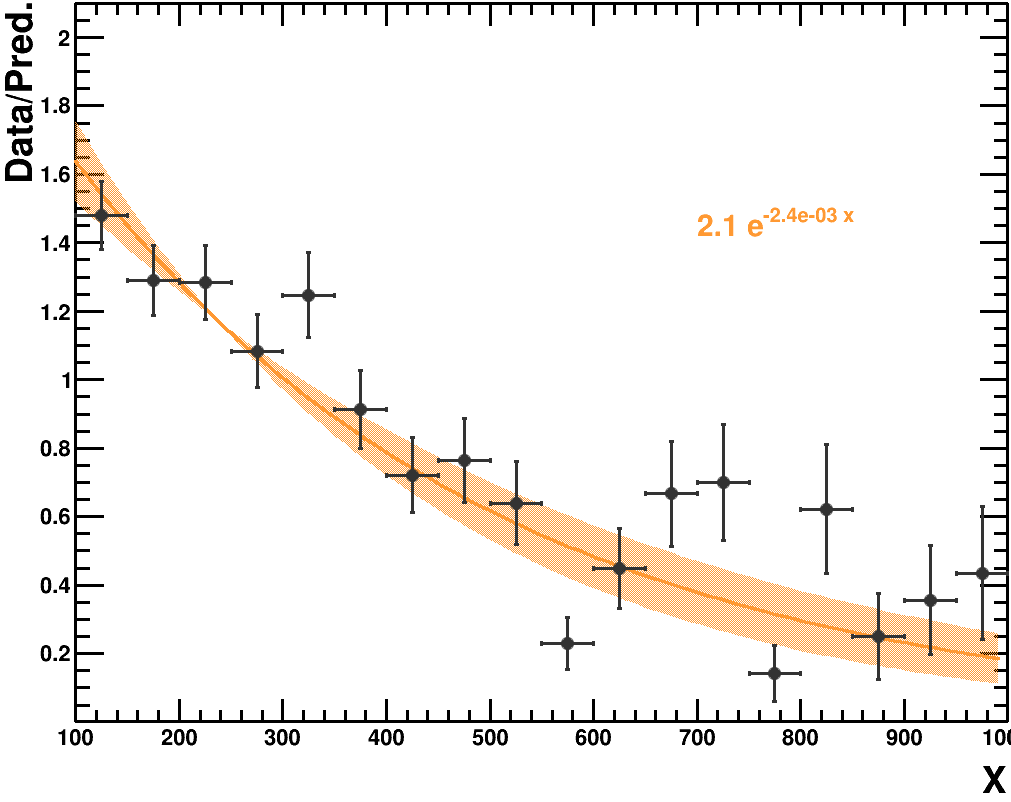
\includegraphics[width=0.48\textwidth]{plots/bkg_modelling/toy_fit_poor.png}
        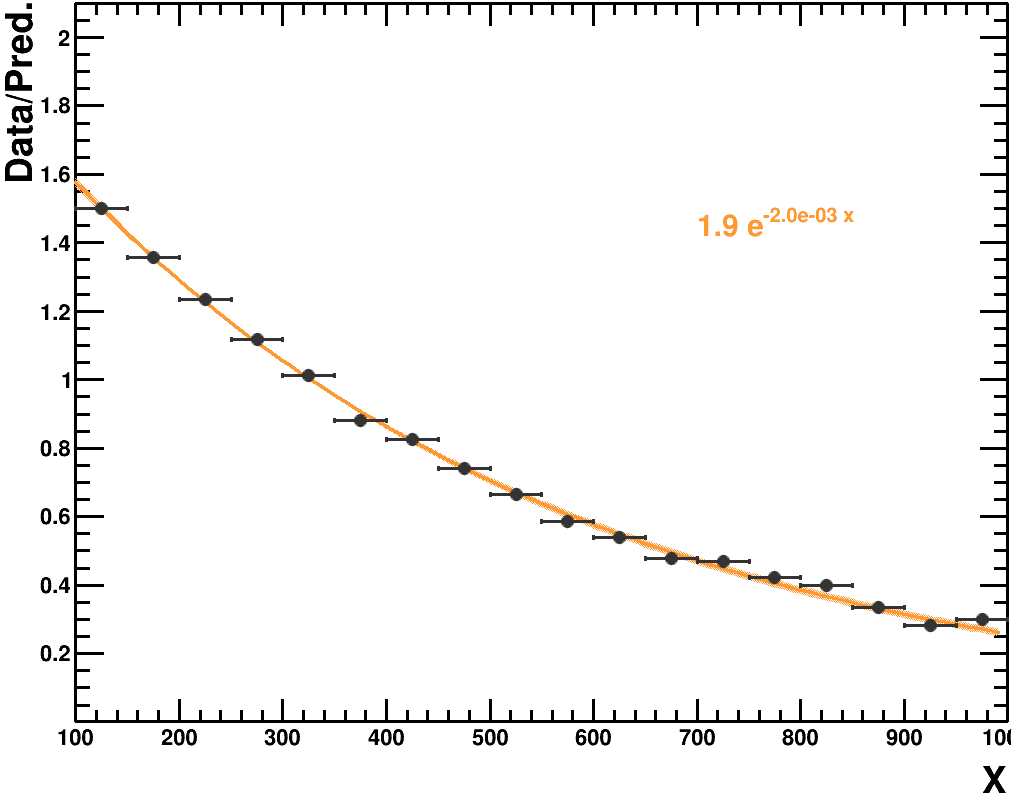
\includegraphics[width=0.48\textwidth]{plots/bkg_modelling/toy_fit.png}
      \end{subfigure}
     \caption{A toy example, generated randomly with two different coefficients of exponential function labeled as data and MC for 1000 (left), and 100000 (right) events.
     (a) Showing correction from NN reweighting and fit function with their uncertainty, (b) reweighting function from NN training and derived uncertainty,
     (c) fit function and the confidence interval at 68\%}
      \label{fig::unc_rew}
  \end{figure}

The given example in Figure~\ref{fig::unc_rew} shows a comparable effect of statistical error on the both NN, and fit modeling for background estimation. Therefore, the statistical errors on the derived reweighting factors are propagated through the MC dropout method, to the \ttbar +jets prediction and their impact are considered as nuisance parameters in the likelihood fit.

\begin{figure}[!htb]
    \centering
      (a)
      \begin{subfigure}[t]{\textwidth}
          \centering
          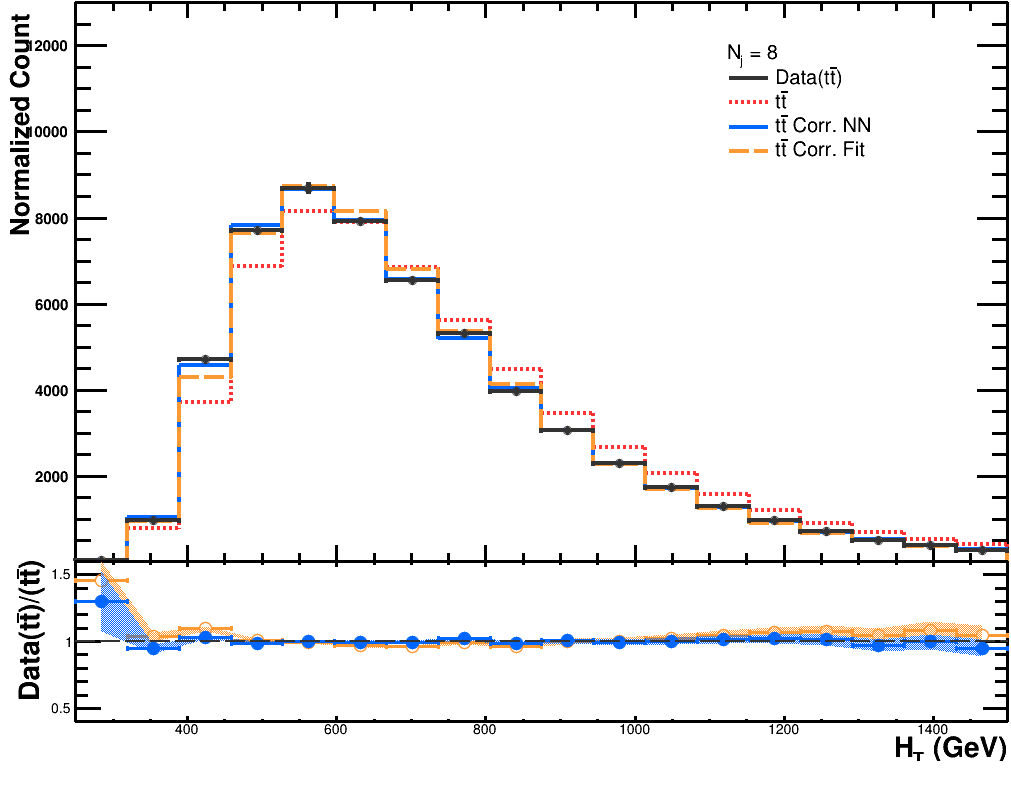
\includegraphics[width=0.48\textwidth]{plots/bkg_modelling/nn_rew_unc_real/val_8.png}
          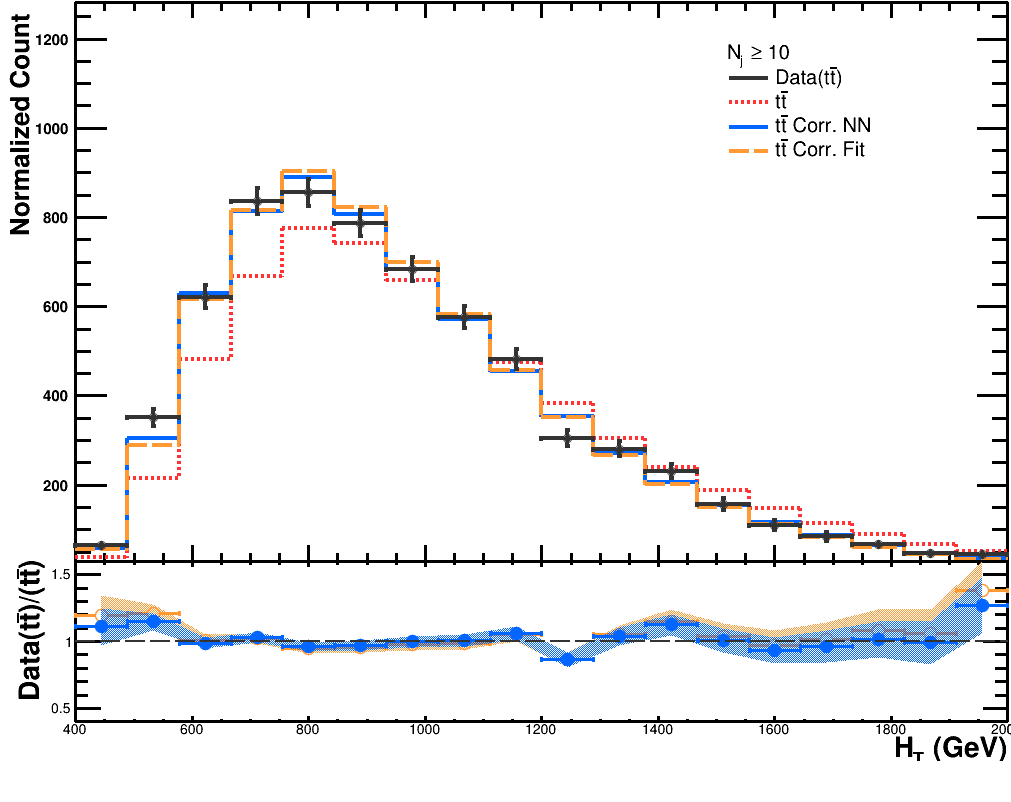
\includegraphics[width=0.48\textwidth]{plots/bkg_modelling/nn_rew_unc_real/val_geq10.png}
      \end{subfigure}
      (b)
      \begin{subfigure}[t]{\textwidth}
        \centering
        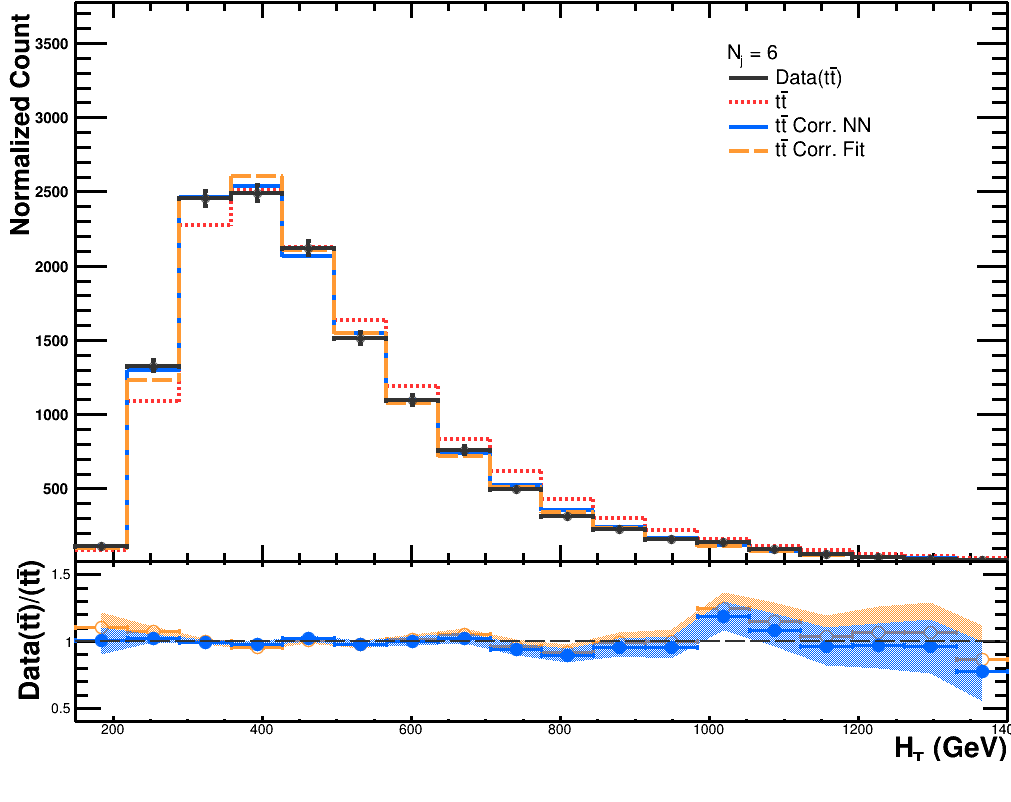
\includegraphics[width=0.48\textwidth]{plots/bkg_modelling/nn_rew_unc_real/val_2los_6.png}
        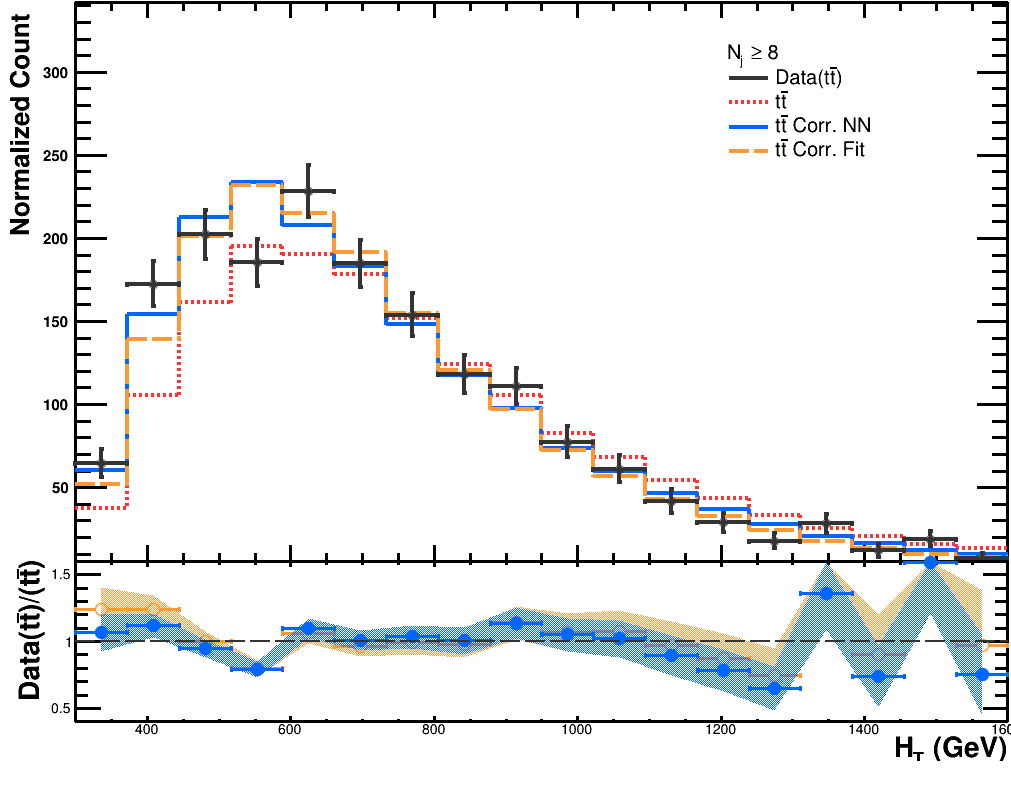
\includegraphics[width=0.48\textwidth]{plots/bkg_modelling/nn_rew_unc_real/val_2los_geq8.png}
      \end{subfigure}
     \caption{$H_{T}$ distributions with data/MC ratio for before and after correction from NN reweighting and MC dropout method, and fit modeling from two different coefficients of exponential function, and its confidence interval at 68\% (a) 1L, (b) (2LOS) channel, and left exclusive 8j(6j), right at least 10j(8j) jets multiplicities selections.}
      \label{fig::unc_rew_real}
  \end{figure}

